\chapter{Simulation, Indistinguishability, and the Necessity of PKI}
\section{On Impossibility Results}
\textbf{Recap and context.} Last lecture, we proved a possibility result showing that, under a
list of assumptions, there is a state machine replication (SMR) protocol satisfying the two
properties that we care about, consistency and liveness. We did this by first reducing the
multi-shot SMR problem to the single-shot Byzantine broadcast problem (i.e., showing how
to build a good protocol for the former from one for the latter), and then presenting the
Dolev-Strong protocol, which guarantees termination, agreement, and validity the Byzantine
broadcast problem with any number of Byzantine nodes.\\
Beginning with this lecture and continuing in Lectures 4–6, we’ll switch our focus from
possibility results to impossibility results (before returning to a possibility result for the
Tendermint protocol in Lecture 7). That is, we’ll identify sets of assumptions under which
there are no protocols that satisfy all the properties that we want. This lecture revisits
the Byzantine broadcast problem from Chapter 2 and proves the “FLM impossibility result”,
which states that, under assumptions incomparable to the ones we made for the Dolev-Strong
protocol, there is no protocol that satisfies all of termination, agreement, and validity. There
are several reasons to spend some quality time with this impossibility result:
\begin{enumerate}
    \item It’s part of the distributed computing canon, and has a super-cool proof.
    \item It highlights the importance of cryptographic and trusted setup assumptions (like the
PKI assumption from Chapter 2).
    \item It introduces two recurring themes in proofs of impossibility results in distributed
computing: the idea of an adversary, who performs a simulation of one or more honest
nodes, and the idea of indistinguishability (in which an honest node  can’t distinguish between different worlds in which different behavior
would be expected).
\end{enumerate}

\textbf{Digression: The point of impossibility results.} Theory is great for proving possibility
results, as we saw last lecture with the Dolev-Strong protocol. But arguably, theory might be
even more uniquely suited for \textit{impossibility} results that delineate what computers, algorithms,
and protocols cannot do.
Thinking back on the history of computer science, perhaps the first academic computer
science paper ever was Alan Turing’s 1936 paper that introduced the Turing machine model
of computation[5]. The main result of that paper was an impossibility result showing that
computers will never be able to solve the halting problem. Thus,  impossibility results have
been part of the fabric of computer science literally from day zero as an academic field.
A somewhat more modern example would be the development of \textit{NP}-completeness, which
explains why certain computational problems appear unsolvable by efficient algorithms. Distributed computing is another part of computer science that is defined in part by its deep
and illuminating impossibility results. A lot of the richness of distributed computing as an
academic discipline lies in the subtle curvature of the frontier between what can and cannot
be done (as a function of exactly which assumptions you make).
Impossibility results seems depressing. What are they good for? The point of an impossibility result is definitely not for some academic in an ivory tower to scold someone that
they can’t or shouldn't attempt to solve some problem. No matter what theorems I prove in
these lectures, people are not going to keep building new blockchain protocols and putting
them out into the world (as they should). Rather, an impossibility result teaches you why
you can’t always have everything that you want, and about the compromises that are going
to be required when you tackle a problem.
For example, if you compare the major blockchain consensus protocols (sometimes called
“layer-1s”), you’ll see that none are perfect, and each has its own disappointing weaknesses.
You might then wonder: “Why shouldn't I, or some other super-smart person, design one
protocol to rule them all, with all the good points and none of the bad points of other
protocols?” An impossibility result can inform us that, unfortunately, no matter how smart any
of us might be, such a protocol does not exist. It also provides you with a lens through
which to evaluate and compare different blockchain protocols and the different compromises
they (inevitably) make—for example, learning to identify which protocols “favor safely over
liveness” or vice versa (more on this in later lectures).
Finally, an impossibility result can also indicate that you’re working in too demanding
a model, with too few assumptions. For example, the FLP impossibility result (covered in
Lectures 4–5) rules out good consensus protocols in the extremely demanding “asynchronous model,” and this result will guide us toward the definition of the “partially synchronous model” in Lecture 6. (Whereas without the FLP impossibility result, it’s not clear anyone
would have bothered to write down that model.) As we’ll see, the partially synchronous
model will be the perfect sweet spot between more extreme models—its assumptions are
weak enough that it forces you to design protocols that really are useful in the real world,
yet strong enough to escape the FLP impossibility result and allow for provable guarantees. That's the
reason we are spending time on these
impossibility results they
tell us when trade-offs are absolutely
unavoidable and then we can understand
different consensus protocols as taking
different approaches towards these necessary
trade-offs.



\section{The FLM Impossibility Result}
\subsection{The Byzantine Broadcast Problem}
Recall from Chapter 2 the definition of and goals for the Byzantine broadcast problem (and
see that lecture for further discussion). There is a set $\{1, 2, 3, \cdots, n\}$ of nodes.
The sender has a private input $v^* \in V$. (For this lecture’s impossibility result, we’ll only
need to use set $V = \{0, 1\}$.)\\
The goal is to design a protocol with three properties:\\
\nt{
\begin{center}
    \textbf{Desired Properties of a Byzantine Broadcast Protocol}
\end{center}
\begin{enumerate}
    \item \textbf{Termination: }Every honest node $i$ eventually halts with some output $v_i \in V$.
    \item \textbf{Agreement: }All honest nodes halt with the same output (whether or
not the sender is honest).
    \item \textbf{Validity: }If the sender is an honest node, then the common output of
the honest nodes is the private input $v^*$ of the sender.
\end{enumerate}
}

\subsection{Statement of the Impossibility Result}
The impossibility result in this lecture was first established by Pease, Shostak, and Lamport [3] (the same authors from the “Byzantine generals” paper mentioned last lecture, with their names in a different order). We’ll present a later (super-slick) proof by Fischer, Lynch,
and Merritt[1]. For the theorem statement, recall that we use $f$ to denote a known upper
bound on the maximum number of Byzantine nodes, where a Byzantine node can deviate
from the intended protocol in arbitrary ways. (The bigger the $f$, the harder it is for honest
nodes to not get confused and achieve consensus.)
\thm{}{
\textit{In the synchronous model with $f \geq \frac{n}{3}$, there is no Byzantine broadcast protocol that satisfies termination, agreement, and validity.
}}
This is, Byzantine broadcast is possible in the synchronous model only if more than two thirds of the nodes are honest and correctly follow the protocol. Here “synchronous model” is the same model of communication that we used for the Dolev-Strong protocol in the last
lecture—all nodes share a global clock, and every message sent in a time step arrives at its
recipient prior to the beginning of the next time step.

\subsection{Cryptography and Trusted Setups Matter!}

Looking at the statement of Theorem 3.2.1, you should have a question: Didn't we just
(in Chapter 2) learn a protocol (the Dolev-Strong protocol) that does solve the Byzantine
broadcast problem (in the synchronous model) no matter how many Byzantine nodes there
are? Yes we did! But neither the proof from last lecture nor the forthcoming proof of
Theorem 3.2.1 are incorrect. The reason there’s no contradiction is that the two results apply
under slightly different sets of assumptions (in particular, different cryptographic/trusted
setup assumptions). So, as we go through the proof of Theorem 3.2.1 in the next section,
your need to keep an eye out for any steps in the proof that wouldn't apply to the
Dolev-Strong protocol (and there must be some, since that protocol escapes the impossibility
result). We’ll discuss this point in Section 3.4.


\subsection{Two Simplifying Assumptions}
To keep the length of this lecture reasonable, let’s make two simplifying assumptions (both
of which can be removed with a bit more work). First, let’s focus on deterministic protocols (with no random coin flips). Allowing randomization doesn't really save you from the impossibility result (see [2]), but let’s not worry about it further. Second, let’s focus on the
simplest possible case of the impossibility result, with $n = 3$ and $f = 1$ (three nodes, one
of which might be Byzantine). Your first reaction might be that this assumption trivializes
the result, but the truth is the exact opposite—this special case already captures all of the
complexity and nuance of the general impossibility result. A good homework problem is
to extend this lecture’s argument for the special case of $n = 3$ and $f = 1$ to a proof of
Theorem 3.2.1 in its full glory. One approach is to use a reduction—that is, to show how
to use a protocol that allegedly solves the Byzantine broadcast problem for some $n$ and
$f \geq \frac{n}{3}$ to build a different protocol that solves the $n = 3$ and $f = 1$ case (which would
be a contradiction). Alternatively, the proof in the next section can be reworked to directly
apply to your favorite choice of $n$ and $f \geq \frac{n}{3}$.

\subsection{Some Vague Intuition}
Before getting to the formal proof of Theorem 3.2.1, let me give you some intuition about
why the result might be true, and what’s fundamentally driving the magical threshold of
$\frac{n}{3}$. (By the way, if you skip the proof, don’t forget to read Section 3.4 for a discussion of
why the Dolev-Strong protocol doesn't contradict Theorem 3.2.1.) Warning: the intuition could
be somewhat vague. The super-slick proof in Section 3.3 more or less encodes this intuition,
though there is some distance between them.\\
\begin{figure}[h]
    \centering
    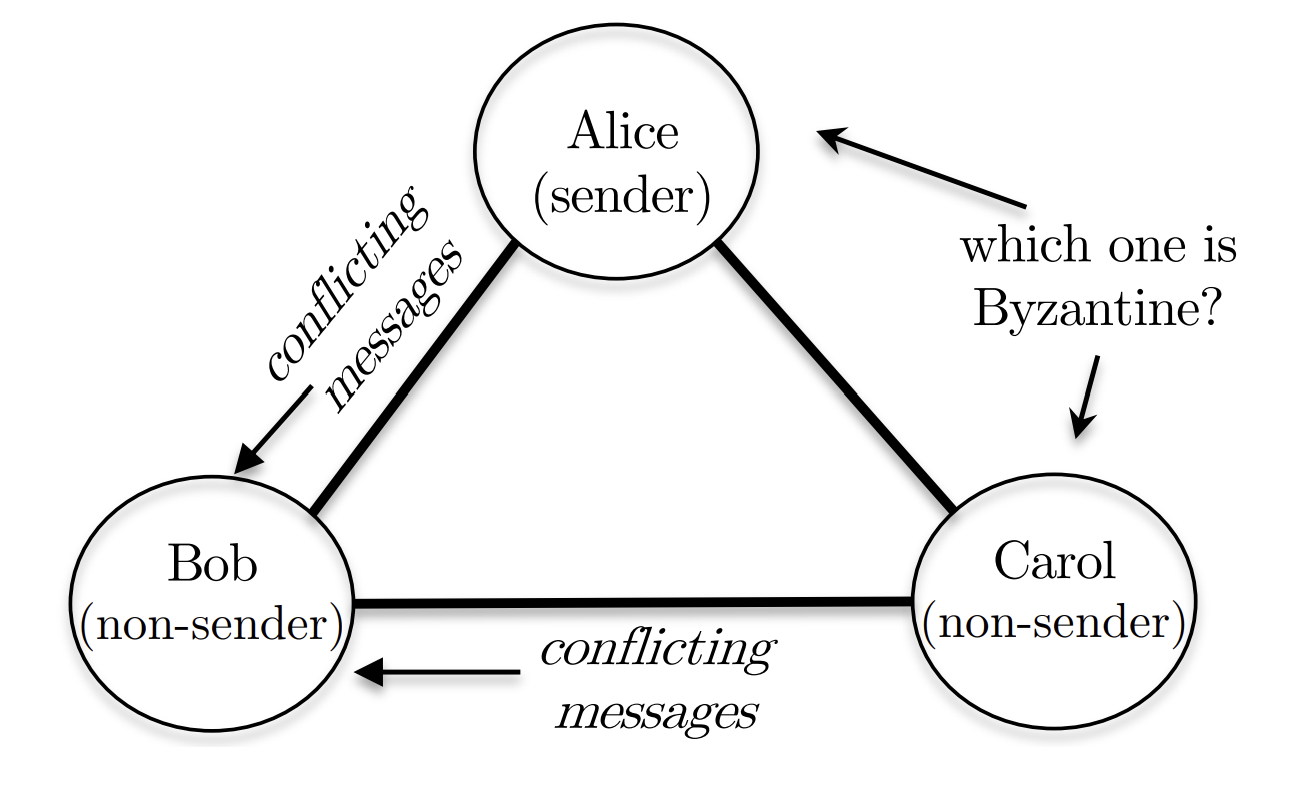
\includegraphics[scale = 0.5]{figures/f3.png}
    \caption{Vague intuition for Theorem 3.2.1. Bob can’t tell if Alice (the sender) is Byzantine
and Carol is honestly echoing her messages or if Carol is Byzantine and trying to frame
Alice.}
    \label{fig:mesh1}
\end{figure}\\
Think of a set of three nodes, call them Alice, Bob, and Carol, shown as vertices in
Figure 3.1. The edges in the figure indicate that each of three nodes knows about and can
communicate with the other two nodes. Assume that Alice is the designated sender.
The basic idea is that one node may have enough information to deduce that one of the
other two nodes is Byzantine but not enough to deduce which one it is. For example, assume
the role of Bob. He might hear conflicting information from Alice (the sender) and Carol
(the other non-sender), for example if Carol is supposed to repeat to Bob any messages she
received from Alice. One plausible scenario is that Carol is honestly echoing the messages
she heard from Alice, but Alice is Byzantine and sending conflicting messages to Bob. But
it’s also totally possible that Alice is honest and sent out consistent information, but Carol
is Byzantine and attempting to frame Alice. Unable to determine who is to blame, Bob
doesn’t know what he should output. (Whereas if $n = 4$ and $f = 1$, Bob could plausibly
figure out the right output by resorting to some type of majority vote over the other three
nodes.)
If you’re really on top of things, you might be suspicious of this informal argument (in
particular, of Carol’s ability to frame Alice) and have an inkling about why an argument
of this type might not apply to the Dolev-Strong protocol. In any case, spot the inevitable
step(s) of the proof in the next section that doesn’t apply to the Dolev-Strong protocol!

\section{The FLM Proof of Theorem 3.2.1}
\subsection{Preamble (Optional)}
The FLM proof of Theorem 3.2.1 is impressively clever—almost like they already knew the
result was true and wanted to back out the slickest proof possible. (Actually, maybe that’s
exactly what they were doing—recall that the theorem was proved earlier in [3].) No one
who sees this proof thinks it would be easy to come up with, and it’s normal to not grok it
the first time you see it. On the very first reading, your main goal should be convincing yourself that it’s correct. With some repeated readings and rumination, you’ll be able to internalize it.\\


\noindent
\textbf{The challenge of impossibility results.} The main reason that impossibility results in
computer science are so challenging is the richness of the design space—you need to rule
out any possible solution, no matter how creative or crazy. This is exactly what made
Turing’s impossibility result [5] such a breakthrough—no algorithm, present or future, no
matter how wild, could ever solve the halting problem.
Some issues can make impossibility results for distributed protocols difficult.
For example, suppose we try to prove Theorem 3.2.1 by contradiction. That is, we assume
that the theorem is false and that there in fact a protocol (call it $\pi$) for the Byzantine
broadcast problem with $n = 3$ and $f = 1$ guaranteed to satisfy termination, agreement, and
validity. If we can derive a contradiction (showing that our initial assumption is false), we’ll
have completed the proof. Here’s the thing, though: we have no idea what $\pi$ looks like, as
it could be arbitrarily crazy event-driven piece of code. One sort of trivial thing we can
say about $\pi$ is that it is designed to work in the $n = 3$ case and we're in the permissioned setting so that means if you're a node running $\pi$ basically you're going to know about two IP addresses different than yours
and these are the two nodes you should be expecting to hear messages from (you're not expecting your messages from anyone other than these two IP addresses)
and you should also feel free to send messages to those nodes whenever you desire. How can we write down a single
argument that somehow works simultaneously for all of the infinitely possible $\pi$’s?\\

\noindent
\textbf{Simulation and indistinguishability.} There is one thing we can do in the proof that
uses the assumed protocol $\pi$ in a generic way: run it! That is, we (or an adversary) can
imagine deploying it on one or more nodes and then seeing what happens. (Proofs in
theoretical computer science often use algorithms in this “black-box” way. E.g., reread any
NP-completeness proof that you might have seen in the past.) This idea of “simulation”—in
our case, of hypothetical honest nodes by a devious Byzantine node—is one of the two key
themes to look for in the FLM proof of Theorem 3.2.1.\\
The second theme of the proof is “indistinguishability,” which we alluded to in the vague
intuition given in Section 3.2.5. Indistinguishability refers to a catch-22 situation faced by an
honest node, in which the node does not have enough information to figure out which of
two plausible scenarios is the actual reality.
\ex{The example for this case is when we had alice,
bob and carol. We were thinking of alice as the sender and we were  playing the role of bob an honest
non-sender and we talked about how you know, on the one hand alice might be byzantine send out conflicting
information and on the other hand carol might be the byzantine one and might try to frame alice and convince bob that alice is
byzantine when in fact it's carol the byzantine one. So you know what this is trying to say, is that you
know bob is now in this sort of catch-22 sort of impossible situation. It really can't distinguish between whether alice is the byzantine one or whether it's carol based on the messages received
and conceivably bob's appropriate behavior with respect to validity and agreement is going to depend on which of
those two situations is the case and this is what makes consensus hard. Honest nodes find themselves in this catch-22,
they might be in world A, they might be in world B and they can't distinguish which one they're in and if the sort of requirements demand different behavior of that node in the two different settings the node gets stuck and it can only do one thing. It's going to be right in one of the worlds and it's going to be wrong in the other world.}\\
If validity and/or agreement demand different
outputs in the two cases, then the node $i$s hopelessly stuck (whatever it outputs, it will be
an incorrect output for one of the plausible scenarios).
With a specific protocol, we can start imagine ways in which a Byzantine node might
trap an honest node into a catch-22 situation (along the lines of Section 3.2.5). But how can
we do it in a generic way, that applies no matter what $\pi$ is?

\subsection{The Hexagon (a Thought Experiment)}
Next is the really, really ingenuous step of the Fischer-Lynch-Merritt proof, which involves a
thought experiment carried out on a 6-cycle of nodes (a “hexagon”). (Once you've convinced
yourself that this thought experiment makes sense, the rest of the proof won’t be too bad.)
The basic idea is to effectively make two copies of each of Alice, Bob, and Carol, in
order to force them to participate simultaneously in multiple worlds that demand different
things of them. Accordingly, we’re going to buy six machines and deploy an allegedly correct
Byzantine broadcast protocol $\pi$ on each of them.\\
To make sense of this idea, let’s be clear on the inputs that the protocol $\pi$ is expecting
to find when it’s first fired up on some node $i$ (in a locally stored initialization file, if you
like):\\
\begin{enumerate}[label=(\alph*)]
    \item the names and IP addresses of two other nodes (recall the protocol $\pi$ is designed for
the case of $n = 3$),
    \item among node $i$ and the two other nodes, which one is the sender (there should be exactly
one sender),
    \item if node $i$ is the sender, its private input.
\end{enumerate}

The designer of the protocol $\pi$ surely had in mind a scenario in which the initialization
files at $i$’s two neighbors (call them $j$ and $k$) list the nodes $i$, $k$ and $i$, $j$, respectively—this
would be the case in any bonafide instance of Byzantine broadcast with $n = 3$, and these
are the only cases that $\pi$’s designer is responsible for. However, at least in principle, we
could run the protocol $\pi$ at node $i$ even if $j$’s and $k$’s initialization files did not satisfy
this consistency property. We can’t count on $\pi$ satisfying any properties in this case. For
example, the initialization file inconsistencies might well cause the protocol to run forever.
But because $\pi$ is just a piece of code and node $i$’s initialization file has all the requisite
ingredients, we can nonetheless press play on node $i$ and see what happens.
The hexagon thought experiment exploits the idea above, running six copies of $\pi$ on
machines with inconsistent initialization files (Figure 3.2, with edges indicating pairs of nodes
that know about each other before the protocol starts):
\begin{figure}[h]
    \centering
    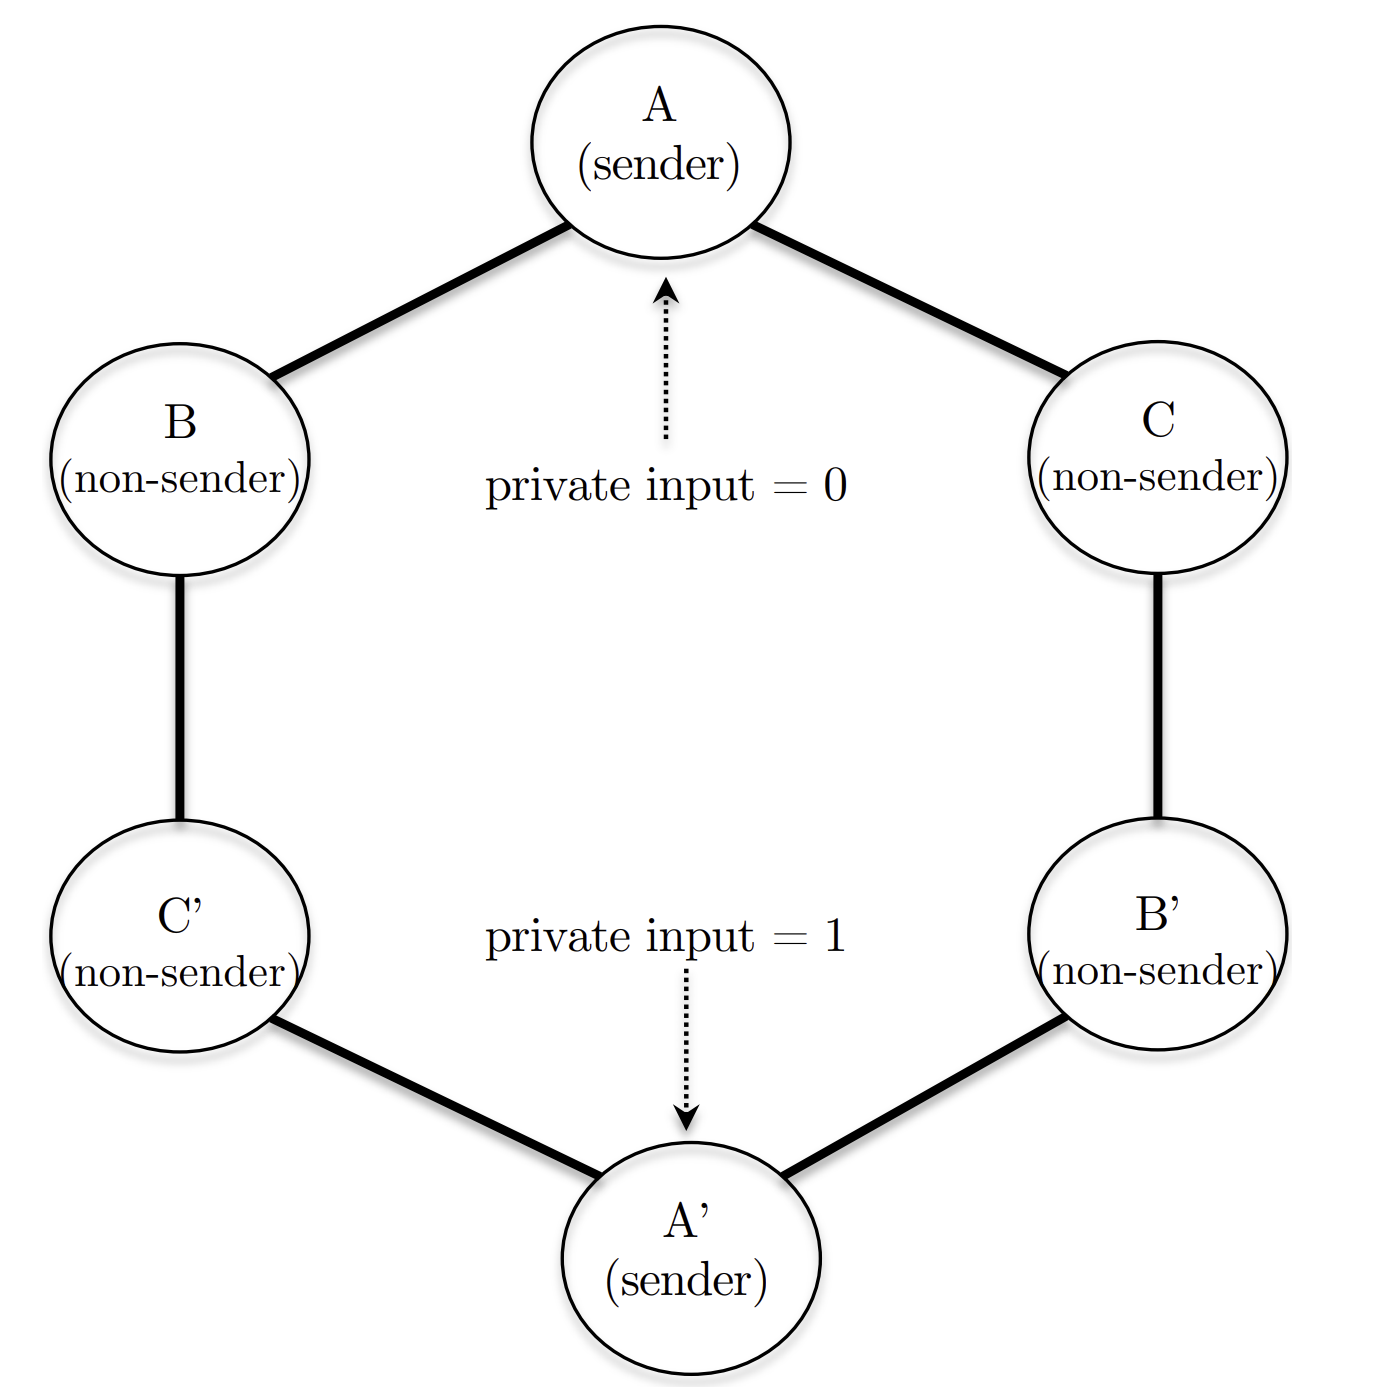
\includegraphics[scale = 0.5]{figures/f4.png}
    \caption{The hexagon thought experiment. Each machine runs the protocol $\pi$ with the
indicated two neighbors (and, if a sender, with the indicated private input).}
    \label{fig:mesh1}
\end{figure}\\


\nt{
\begin{center}
    \textbf{Thought Experiment Instructions}
\end{center}

\begin{enumerate}
    \item Buy a node A and set it up with the following initialization file:
    \begin{enumerate}[label=(\roman*)]
        \item A’s neighbors are the nodes B and C (specified by name and IP address);
        \item A is a sender while B, C are non-senders;
        \item A’s private input is 0.
    \end{enumerate}
    \item Buy a node B and set it up with:
    \begin{enumerate}[label=(\roman*)]
        \item B’s neighbors are the nodes A and C'
        \item A is a sender while B, C' are non-senders. (Think of C' as having the same name as C (e.g., each thinks it’s a real node but it has a different IP address.)
    \end{enumerate}
    \item Buy and setup a node C with:
    \begin{enumerate}[label=(\roman*)]
        \item neighbors A and B'
        \item A is a sender while B' and C are non-senders
    \end{enumerate}
    \item Buy and setup a node C' with:
    \begin{enumerate}[label=(\roman*)]
        \item neighbors A' and B;
        \item A' is a sender while B, C' are non-senders.
    \end{enumerate}
    \item Buy and setup a node B' with:
    \begin{enumerate}[label=(\roman*)]
        \item neighbors A' and C;
        \item A' is a sender while B', C are non-senders.
    \end{enumerate}
    \item Buy and setup a node A' with:
    \begin{enumerate}[label=(\roman*)]
        \item neighbors B' and C'
        \item A' is a sender while B', C' are non-senders;
        \item the private input of A' is 1.
    \end{enumerate}
\end{enumerate}
}

This whole endeavor should seem bizarre. The only point to understand now is that, given
the code of a protocol $\pi$, no one can stop you from buying six machines, installing $\pi$ on each
of them, and setting up their initialization files as above. Because each initialization file has
exactly the information (a)–(c) expected by $\pi$—for all the node knows, it’s participating in
a bonafide instance of Byzantine broadcast with $n = 3$—no one can stop you from pressing
play simultaneously on all six machines. All bets are off about what happens next ($\pi$ was
not designed with this experiment in mind), but no one can stop you from running the
experiment to see what the nodes’ eventual outputs will be.

\subsection{Proof Strategy}
Because the initialization file of each node in the hexagon thought experiment typechecks with the expectations of the protocol $\pi$, you can run the experiment of running $\pi$ simultaneously on all six nodes. But the overall setting in the thought experiment
($n = 6$, not all nodes no about all other nodes) certainly doesn't typecheck with the one $\pi$ is designed
for ($n = 3$, set of nodes common knowledge). Thus any properties that $\pi$ might have in
the latter scenario (e.g., validity) need not carry over to the former scenario (e.g., with two
senders with different private inputs, it’s not even clear what validity should mean). This
point has important consequences for our proof strategy.\\
In our proof, to derive a contradiction, presumably we are going to use the assumptions that $\pi$ satisfies termination, agreement, and validity. (Achieving any two of the three
properties is easy, so there’s no way to prove an impossibility result without using all three
assumptions.) How are we going to use the assumed properties of $\pi$ in the proof, given that
we can’t appeal to them directly in the hexagon thought experiment?\\
To build a bridge between the hexagon experiment (where $\pi$ has no guarantees) and bonafide three-node instances of Byzantine broadcast (where $\pi$ satisfies termination, agreement,
and validity), we’re going to show that the hexagon effectively encodes three different three node Byzantine broadcast instances. In each of these instances, agreement or validity will impose a constraint on the outputs of a pair of nodes, and these constraints will carry over to
the hexagon. We’ll see that the three constraints are mutually incompatible, contradicting
the fact that the hexagon thought experiment must have some well-defined output. In our example, all 6 nodes eventually output 0 or 1($\pi$ satisfies termination).

\subsection{Byzantine Broadcast Instance 1}
Let’s see the first instance of Byzantine broadcast that is effectively “embedded” in the
hexagon through experiment. Consider the instance shown in Figure 3.3(a), with a Byzantine sender (node $X$) and two honest non-senders (B and C'). As a bonafide instance of Byzantine broadcast (with $n = 3$ and one Byzantine node), we can appeal to the promised
guarantees of the assumed protocol $\pi$, specifically its termination and agreement properties
(validity is irrelevant because the sender is Byzantine). Remember what these properties
say: no matter what a Byzantine node does, no matter how crazy its strategy, the honest
nodes must eventually terminate, and upon termination output the same value.
Intuitively, the protocol $\pi$ must be robust to $X$ sending out conflicting messages. But
given that we know nothing about how $\pi$ works, how can we know which messages might
confuse the nodes that are running $\pi$ honestly? Could there be a generic “send conflicting
messages” strategy for $X$ that applies to every possible protocol $\pi$?
Here’s one crazy strategy that the Byzantine node $X$ in Figure 3.3 could do:
So this is where this will be the first appearance of the simulation idea in this proof. The adversary is
going to simulate the protocol $\pi$, actually it's going to simulate four copies of the protocol $\pi$.
So why four copies? Well it's going to be the four machines in the thought experiment, the four machines in the six-cycle other than B and C'. So that's going to be the chain starting with machine A running as a
sender with input zero. It's going to include the non-senders C and B' and then the sender with input 1:
$$A \leftrightarrow C \leftrightarrow B' \leftrightarrow A'$$

In the hexagon thought experiment, in which A', C, B' and A' run $\pi$ honestly with the
initialization parameters specified in Section 3.3.2. (Remember, simulation is one of the two
key themes of this proof.) Think of it this way: The Byzantine node $X$ spins up four virtual
machines on its node, each running a separate copy of $\pi$ with the appropriate initialization
parameters. The Byzantine node monitors the progress of each copy of $\pi$. Whenever $\pi$ instructs the virtual machine masquerading as A to send a message to A’s neighbor B
(which is $X$’s actual neighbor in the Byzantine broadcast instance), node $X$ sends that
message to B (over the communication network). Similarly, any messages $X$ receives from
B (over the communication network) are forwarded to the virtual machine on $X$ that is
running $\pi$ as A. Messages between the virtual machine running as A' and the (actual)
node C' are handled analogously, over the communication network. Finally, whenever one
virtual machine wants to send a message to another one (e.g., messages between the virtual
machines running as C and B'), the Byzantine node $X$ can directly deliver that message
to the destination machine, without ever touching the communication network. In the end,
the Byzantine node $X$ interacts with its neighbor B as if it were the node A in the hexagon
(running $\pi$ honestly with private input 0) and with C' as if it were the node A'
in the hexagon (running $\pi$ honestly with private input 1). This strategy is well defined for any protocol $\pi$
and thus serves as our generic way for a Byzantine node to send conflicting messages.\\
\begin{figure}[h]
    \centering
    \subfloat[\centering Byzantine broadcast instance]{{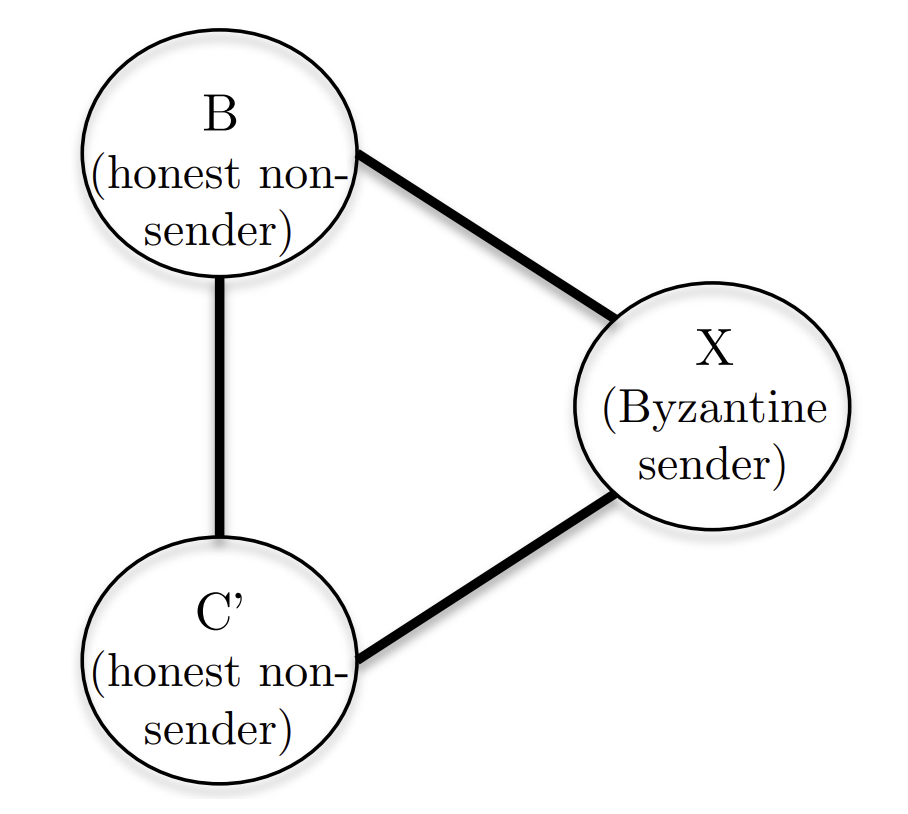
\includegraphics[width=7cm]{figures/f5.png} }}%
    \qquad
    \subfloat[\centering Hexagon thought experiment]{{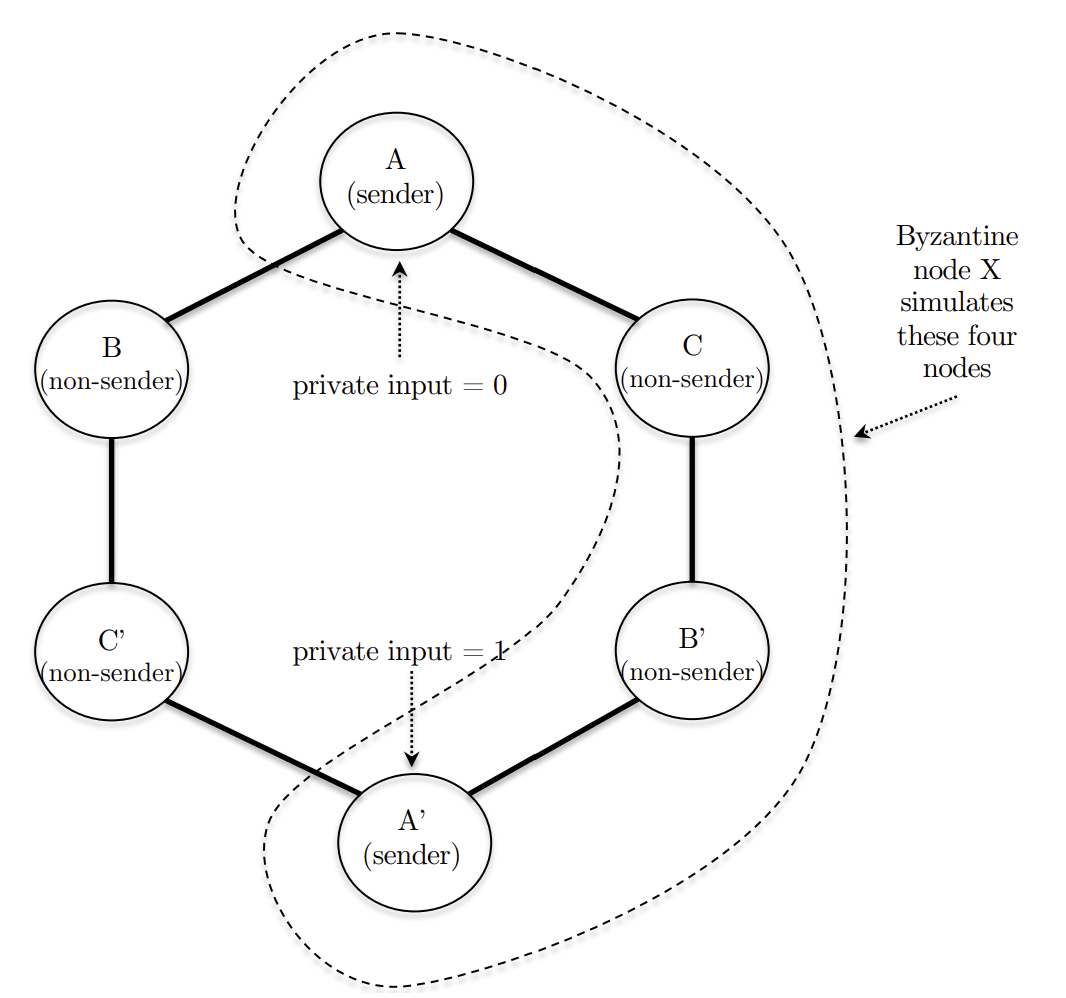
\includegraphics[width=7cm]{figures/f6.png} }}%
    \caption{Left: Byzantine broadcast instance 1 (with $n = 3$ and one Byzantine node).
    Right: by simulating four nodes in the hexagon experiment, the Byzantine node $X$ can
    force B and C' to operate identically in the triangle and in the hexagon. The agreement
    property of $\pi$ dictates that B and C' output the same value.}
    \label{fig:example}%
\end{figure}\\

At this point you should agree that this “simulate four nodes on the hexagon” strategy is
something that the Byzantine node $X$ could do. But what’s the point of this crazy strategy?
The point is that it tricks the honest nodes B and C' to behave exactly as if they were in
the hexagon experiment. That is, because the initialization parameters and the sequences
of messages received by B and C' are exactly the same in the triangle in Figure 3.3(a) (by
construction of $X$’s strategy) and in the hexagon in Figure 3.3(b), they are kept in the dark and they
cannot distinguish which is the actual reality and must operate identically in both cases.
(Remember, indistinguishability is the other key theme of the proof.)

Now we can see how to translate $\pi$’s assumed properties in bonafide Byzantine broadcast instances (like the triangle in Figure 3.3(a), with the above Byzantine node strategy) to properties of its behavior in the hexagon experiment. Specifically, in the triangle, because
$\pi$ satisfies termination and agreement, nodes B and C' eventually output something, and
the outputs must be the same. (This statement is true no matter what strategy $X$ uses.)
Because B and C' operate identically in the triangle (with the specified strategy for $X$) and
in the hexagon thought experiment, the outcome must be the same:

$$\text{In the hexagon thought experiment, the nodes B and C' output the same value.} \quad (1)$$

Good news: If you followed the argument in this section, then you've completed all of the
hard parts of understanding the FLM proof of Theorem 3.2.1. We need to talk through two
more scenarios before arriving at a contradiction, but the pattern of those two arguments
will be the same as this one.

\subsection{Byzantine Broadcast Instance 2}
The first scenario relied on the assumed agreement of the protocol $\pi$. The second and third
ones will rely on validity. Validity applies only with an honest sender, so in these two
scenarios the Byzantine node $X$ will be a non-sender (see the triangle in Figure 3.4(a)).
\begin{figure}[h]
    \centering
    \subfloat[\centering Byzantine broadcast instance]{{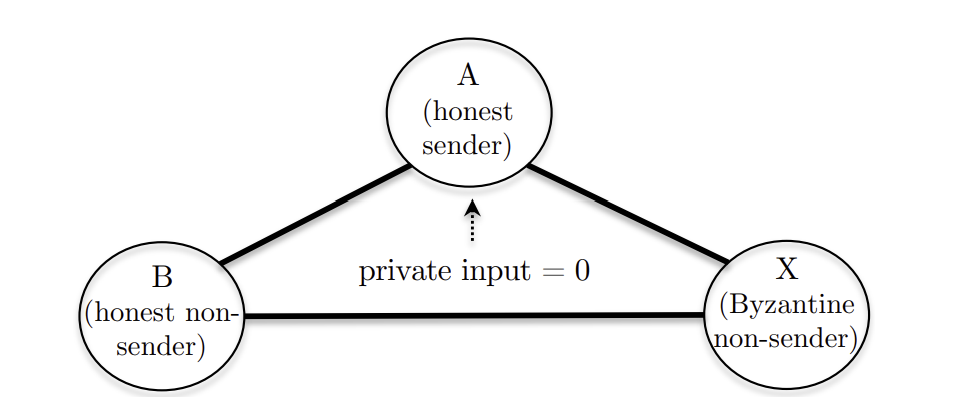
\includegraphics[width=7cm]{figures/f7.png} }}%
    \qquad
    \subfloat[\centering Hexagon thought experiment]{{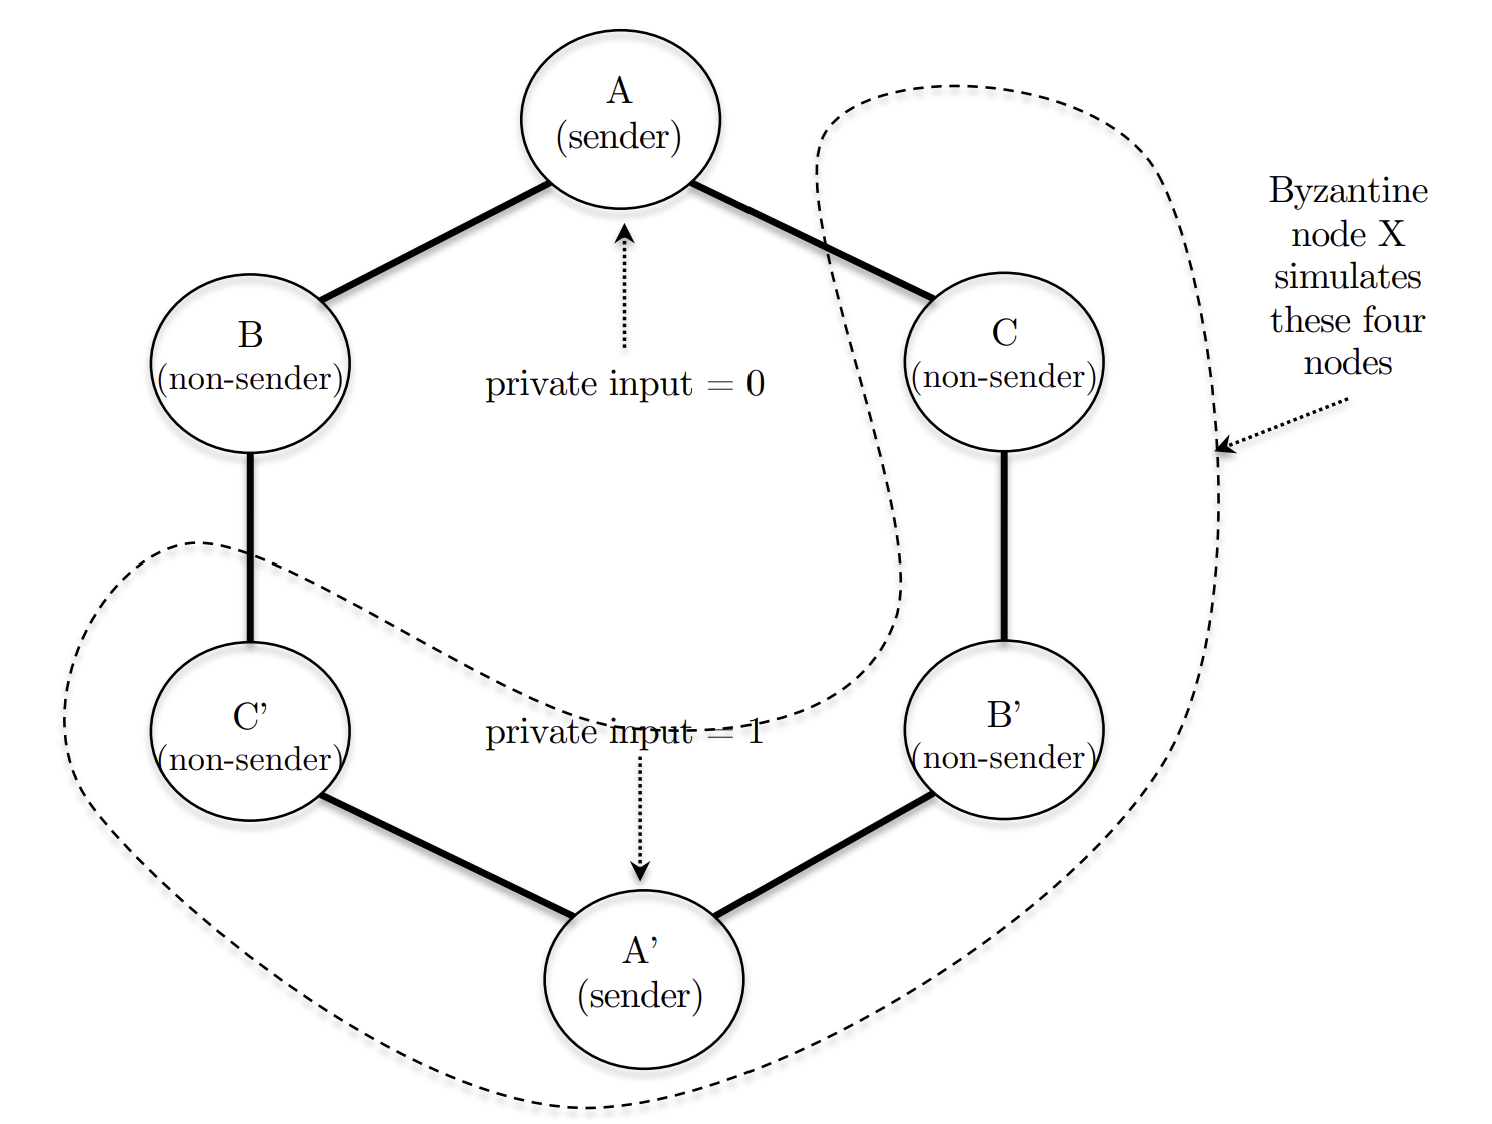
\includegraphics[width=7cm]{figures/f8.png} }}%
    \caption{Left: Byzantine broadcast instance 2. Right: by simulating four nodes in the
    hexagon experiment, the Byzantine node $X$ can force A and B to operate identically in the
    triangle and in the hexagon. The validity property of $\pi$ dictates that A and B both output 0.}
    \label{fig:example}%
\end{figure}\\

The honest nodes A and B in the triangle play the same roles as their namesakes in the
hexagon, and particular the honest sender A has a private input of 0. 
It's going to be the same as before, so we're going to look at the four nodes on the sixth cycle other than the two that are present, so in this case
it's going to be the chain of nodes between C and C' and the adversary is just going to simulate four copies
of the protocol $\pi$. Again it has its computer, it has its four virtual machines. One of those is
running C one is B', one is A' and one is C'. So the the byzantine node $X$ will interact with the honest sender A as
if it was the node C in the thought experiment and it will interact with the honest non-sender B as
if it was the node C' in the thought experiment and then the adversary, the byzantine node $X$ will also be simulating the other nodes of the six cycle A' and B' to ensure that it's faithfully
replicating all of the computation and communication that would be happening in the thought experiment.
To keep the nodes A
and B in the dark as to whether they reside in the triangle or the hexagon, the Byzantine
non-sender $X$ in the triangle runs four copies of $\pi$ (in separate virtual machines) to simulate
the remaining four nodes of the hexagon (Figure 3.4(b)):
$$C \leftrightarrow B' \leftrightarrow A' \leftrightarrow C'$$
That is, the Byzantine node $X$ interacts with the honest sender A as if it were the node C
in the hexagon, and with the honest non-sender B as if it were the node C' in the hexagon
(while also simulating the nodes B' and A' to keep track of which messages C and C'  would
be sending). Because $\pi$ satisfies termination and validity in every bonafide three-node instance of
Byzantine broadcast (like the triangle) with an arbitrary Byzantine node strategy (like $X$’s
simulation strategy), nodes A and B must eventually output 0 (i.e., A’s private input) on
the triangle. By virtue of operating identically in the hexagon experiment (by construction
of $X$’s strategy), those two nodes must also eventually output 0 in the hexagon:
$$\text{In the hexagon thought experiment, the nodes A and B output 0.} \quad (2)$$
Again, the seemingly bizarre simulation strategy by the Byzantine node $X$ is what enables
the transfer of constraints imposed on nodes’ outputs in the triangle to those in the hexagon.


\subsection{Byzantine Broadcast Instance 3}
The third scenario is very similar to the second one, with an honest sender A'
(this time with private input 1), an honest non-sender C', and a Byzantine non-sender X (see the triangle in Figure 3.4(a)).
\begin{figure}[h]
    \centering
    \subfloat[\centering Byzantine broadcast instance]{{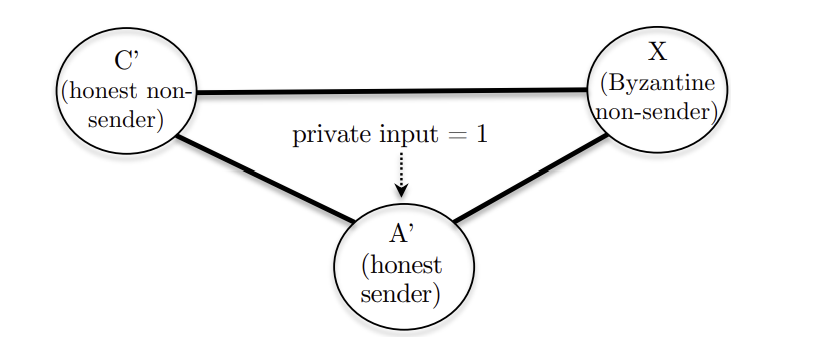
\includegraphics[width=7cm]{figures/f9.png} }}%
    \qquad
    \subfloat[\centering Hexagon thought experiment]{{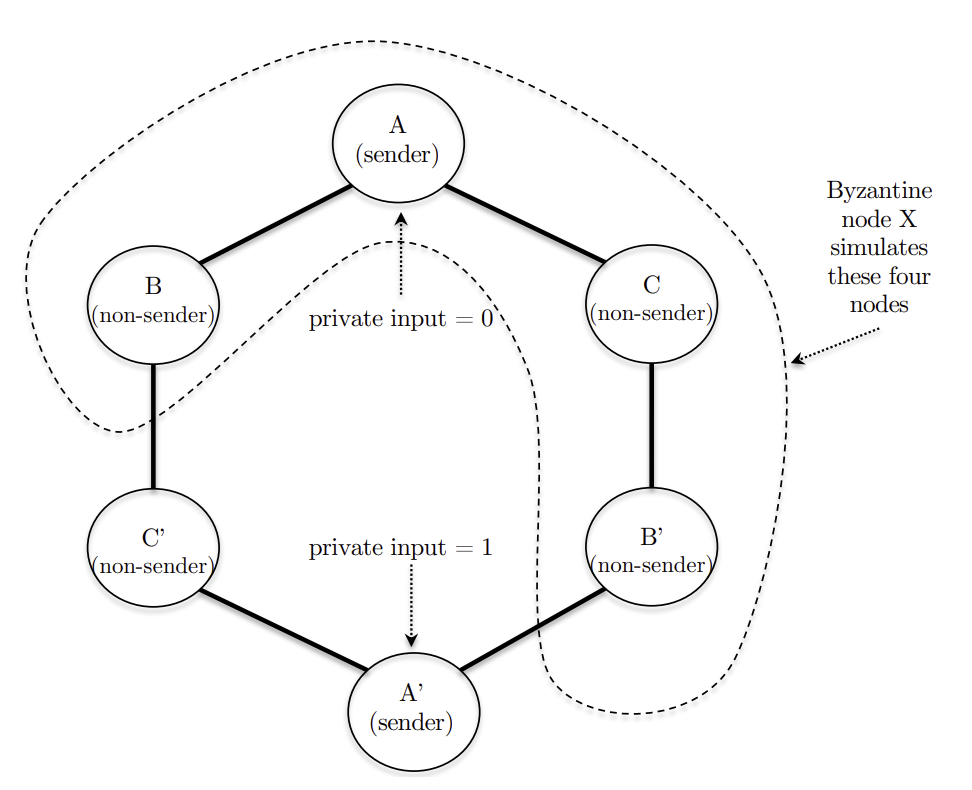
\includegraphics[width=7cm]{figures/f10.png} }}%
    \caption{Left: Byzantine broadcast instance 3. Right: by simulating four nodes in the
    hexagon experiment, the Byzantine node $X$ can force A' and C' to operate identically in
    the triangle and in the hexagon. The validity property of $\pi$ dictates that A' and C' both
    output 1.}
    \label{fig:example}%
\end{figure}\\

To keep the honest nodes A' and C' in the dark as to whether they reside in the triangle
or the hexagon, the Byzantine non-sender $X$ runs four copies of $\pi$ to simulate the remaining
four nodes of the hexagon (Figure 3.4(b))
$$B \leftrightarrow A \leftrightarrow C \leftrightarrow B'$$
interacting with A' as if it were B' and with C' as if it were B.
Because $\pi$ satisfies termination and validity in every bonafide three-node instance of
Byzantine broadcast (like the triangle) with an arbitrary Byzantine node strategy (like X’s
simulation strategy), nodes A' and C' must eventually output 1 (i.e., the private input of
the honest sender A') on the triangle. By virtue of operating identically in the hexagon
experiment (by construction of $X$’s strategy), those two nodes must also eventually output 1
in the hexagon:
$$\text{In the hexagon thought experiment, the nodes A' and C' output 1.} \quad (3)$$

\subsection{Completing the Contradiction}
We looked at three different three-node Byzantine broadcast instances and (appealing to
$\pi$’s assumed guarantees) deduced constraints on the outputs of the honest nodes in each.
We chose a simulation strategy for the Byzantine node in each of these instances to force
the honest nodes to operate identically to how they would act in the hypothetical hexagon
thought experiment defined in Section 3.3.2, thereby transferring the constraints from the three
instances over to hexagon. These constraints (1)–(3) assert that, in the hexagon thought
experiment, nodes B and C' must terminate and output the same thing. B must output 0
and C' must output 1. Whatever the outcome of the hexagon experiment might be (and it
must be something), it can’t possibly satisfy these three mutually inconsistent constraints.
This completes the contradiction, implying that the assumed protocol $\pi$ cannot exist. That
is, there cannot be a Byzantine broadcast protocol with $n = 3$ and $f = 1$ that guarantees
termination, agreement, and validity.

\section{Discussion}
The main result of Chapter 2 is that, in the synchronous model, you can solve the Byzantine
broadcast problem (i.e., with a protocol that satisfies termination, agreement, and validity)
with any number of Byzantine nodes. The main result of this lecture is that, in the synchronous model, you can’t solve the Byzantine broadcast problem if at least one-third of the nodes can be Byzantine. What gives?

\subsection{Resolving the Contradiction}
No prizes for guessing the answer, which appears in the title of this lecture. In Chapter 2,
we introduced the public key infrastructure (PKI) assumption as an extension of the usual
permission assumption. Not only do all the nodes know the names and IP addresses of all the
nodes, but also their public keys. (Each node $i$s assumed to have a distinct public key-private key pair, with the private key known only to the node and the public key known to all.) This is an example of a trusted setup assumption, asserting that a certain computation (in this
case, public key distribution) is done correctly in advance of the protocol’s commencement,
remaining silent on how this computation might actually happen.\\
Our analysis of the Dolev-Strong protocol in Chapter 2 relied on three assumptions: The
permissioned setting (with all node names common knowledge at the start of the protocol),
synchronous setting (reliable message delivery) and the PKI assumption (so that nodes begin
the protocol with the ability to verify each others’ signatures). The proof in Section 3.3 does
not violate the permissioned setting assumption—in all three of the Byzantine broadcast
instances considered, the node set is known to all nodes up front. Neither does it violate
the synchronous setting assumption—it relies only on devious communication strategies for
Byzantine nodes and not on any manipulation of the timing of message deliveries. Thus, by
the process of elimination, we can conclude that Theorem 3.2.1 cannot possibly remain true
under the PKI assumption (if it did, it would contradict what we've already proved about
the Dolev-Strong protocol). Given that the theorem is false with the PKI assumption, the
proof in Section 3.3 must somehow violate that assumption. But now exactly would common
knowledge of nodes’ public keys break the proof?


\subsection{Can We Salvage the Proof?}
For the hexagon thought experiment in Section 3.3.2 to even make sense under the PKI
assumption, we need to add the relevant cryptographic keys to nodes’ initialization files.
The new file format is:\\
\noindent
(I1) the names, IP addresses, and public keys of two other nodes;\\
\noindent
(I2) among node $i$ and the two other nodes, which one is the sender;\\
\noindent
(I3) if node $i$ is the sender, its private input;\\
\noindent
(I4) a public key-private key pair for node $i$ (distinct from those of the other two nodes).\\

\noindent
The most obvious way to modify the thought experiment would then be (see Figure 3.6):
\begin{figure}[h]
    \centering
    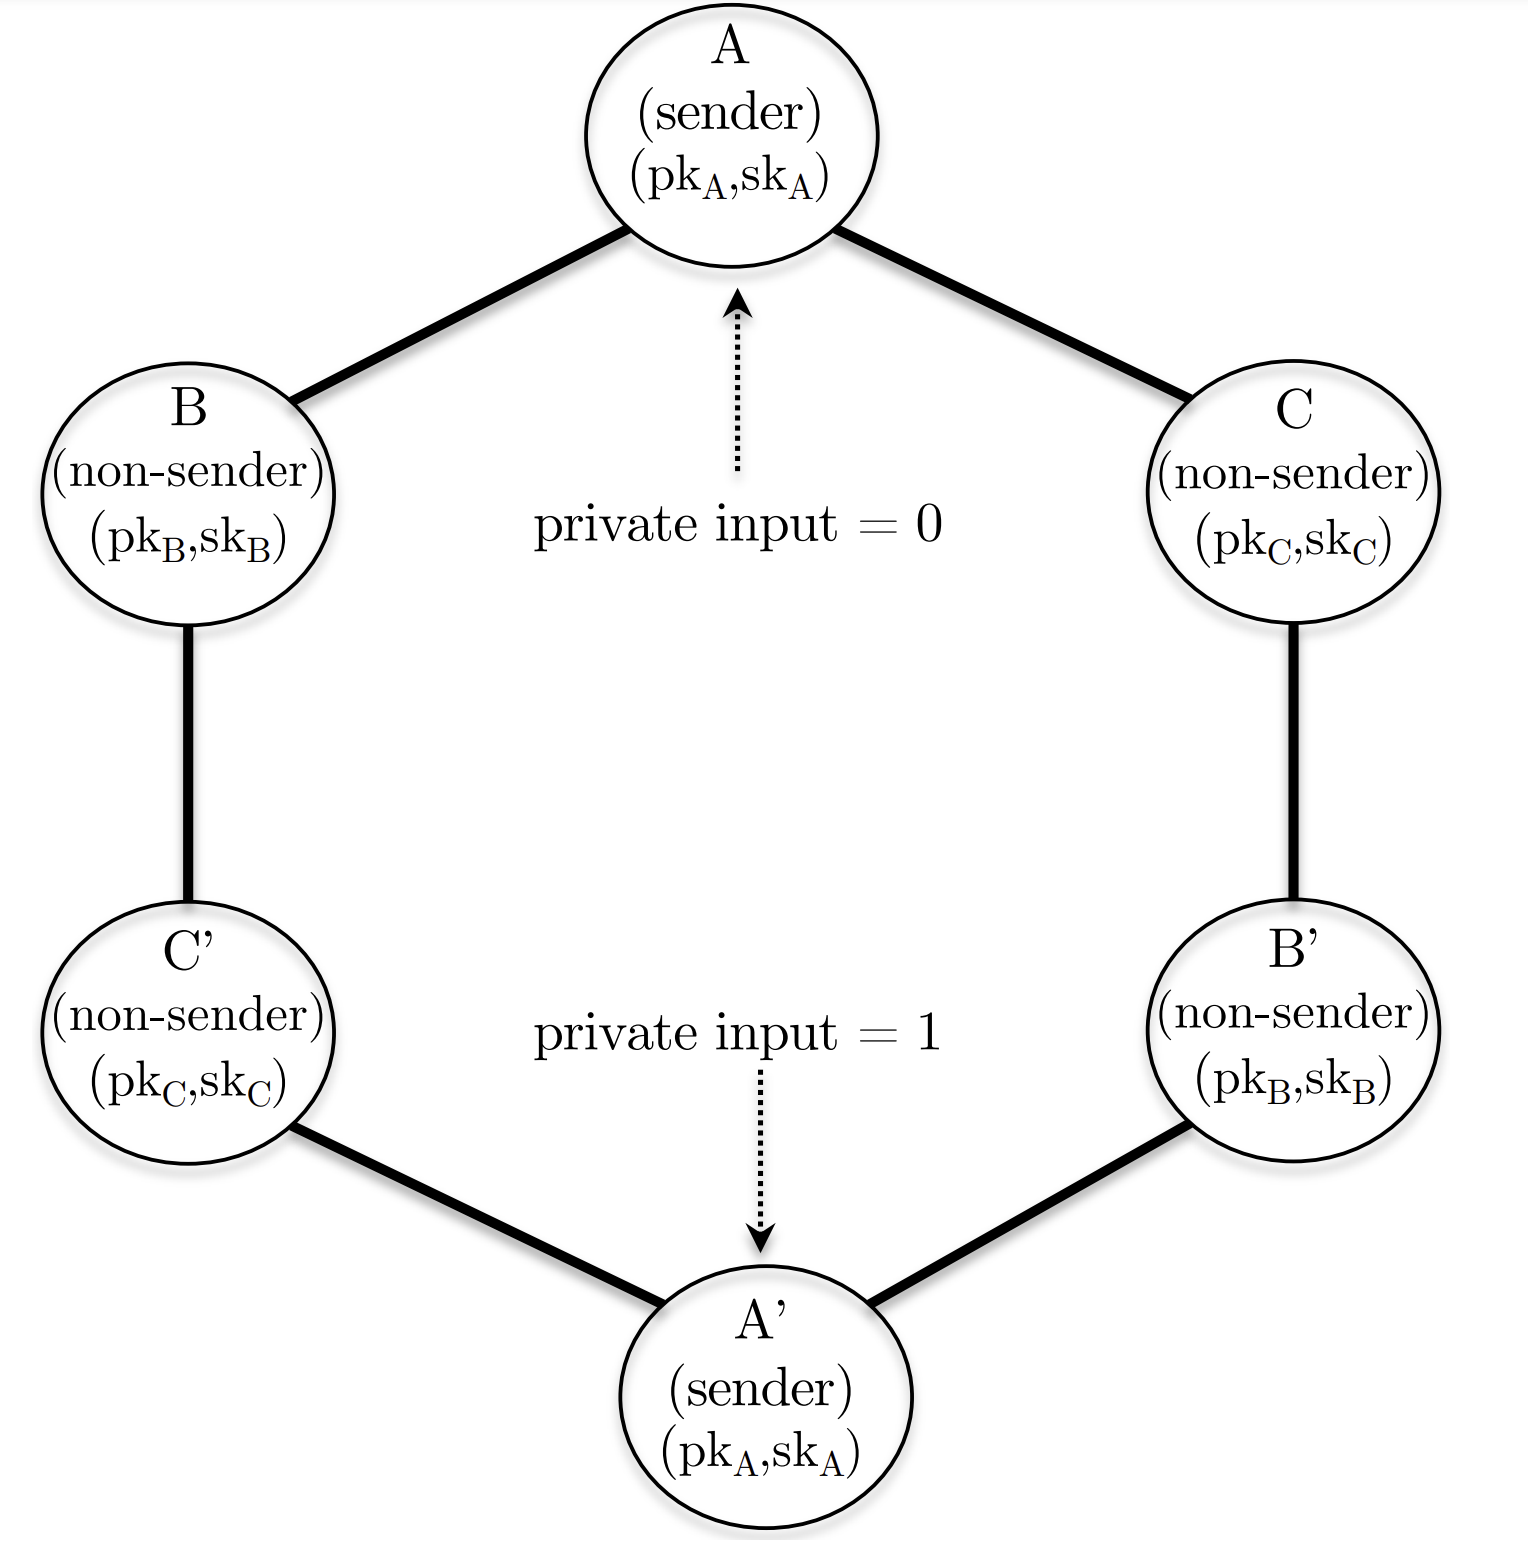
\includegraphics[scale = 0.5]{figures/f11.png}
    \caption{Extension of the hexagon thought experiment to incorporate the PKI assumption.}
    \label{fig:mesh1}
\end{figure}\\

\newpage
\nt{
\begin{center}
    \textbf{Revised Thought Experiment}
\end{center}
\begin{enumerate}
    \item Setup node A with:
    \begin{enumerate}[label=(\roman*)]
        \item neighbors B and C (specified by name, IP address, and public key),
        \item A is a sender while B, C are non-senders,
        \item A’s private input is 0,
        \item a public key-private key pair ($pk_A, sk_A$).
    \end{enumerate}
    \item Buy a node B and set it up with:
    \begin{enumerate}[label=(\roman*)]
        \item B’s neighbors are the nodes A and C',
        \item A is a sender while B, C' are non-senders,
        \item a public key-private key pair ($pk_B, sk_B$). (Think of C' as having the same name and key pair as C (e.g., each thinks it’s the
        real node and has the corresponding credentials) but a different IP
        address.)
    \end{enumerate}
    \item Setup node C with:
    \begin{enumerate}[label=(\roman*)]
        \item neighbors A and B',
        \item A is a sender while B' and C are non-senders,
        \item a public key-private key pair. ($pk_C, sk_C$).
    \end{enumerate}
    \item Setup node C' with:
    \begin{enumerate}[label=(\roman*)]
        \item neighbors A' and B,
        \item A' is a sender while B, C' are non-senders,
        \item a public key-private key pair ($pk_C, sk_C$).
    \end{enumerate}
    \item Setup node B' with:
    \begin{enumerate}[label=(\roman*)]
        \item neighbors A' and C,
        \item A' is a sender while B', C are non-senders,
        \item a public key-private key pair ($pk_B, sk_B$).
    \end{enumerate}
    \item Setup node A' with:
    \begin{enumerate}[label=(\roman*)]
        \item neighbors B' and C',
        \item A' is a sender while B', C' are non-senders,
        \item the private input of A' is 1,
        \item a public key-private key pair ($pk_A, sk_A$).
    \end{enumerate}
\end{enumerate}}
\newpage
Now that we have a well-defined thought experiment with the PKI assumption, let’s try
to replicate the argument in Section 3.3. (The proof hasn't broken yet, but it has to break
somewhere...) The next step is to consider a Byzantine broadcast instance analogous to
the one in Section 4.4 (Figure 3.7(a)) and the strategy for the Byzantine node $X$ in which it
simulates the other four vertices in the revised hexagon experiment (Figure 3.7(b)). Remember
that the point of this strategy is to keep the two honest nodes in the dark as to whether
they reside in the triangle or the hexagon, in which case any constraints we can deduce for
nodes’ behavior in the triangle would carry over to the hexagon.\\
But is the Byzantine node $X$ really in a position to pull off such a simulation? The
assumed Byzantine broadcast protocol $\pi$ might well instruct every node to sign every message
it sends (as in the Dolev-Strong protocol). The adversary $X$ knows its public key-private key
pair ($pk_A, sk_A$) in the Byzantine broadcast instance, as well as the other two public keys $pk_B$
and $pk_C$, but it does not know the other two private keys $sk_B$ and $sk_C$. Thus, while the
adversary is perfectly positioned to simulate the nodes A and A'—the only ones the honest nodes B and C' communication with directly—it cannot sign a message on behalf of nodes B' or C and is therefore unable to simulate them. (Remember our permanent assumptions that
cryptography exists and that a signature for an as-yet-unseen message cannot be forged
without knowledge of the appropriate private key) To sum up, our proof of Theorem 3.2.1 made
crucial use of strategies in which a Byzantine node simulates multiple other honest nodes,
and these strategies become impossible to carry out under the PKI assumption.
\begin{figure}[h]
    \centering
    \subfloat[\centering Byzantine broadcast instance]{{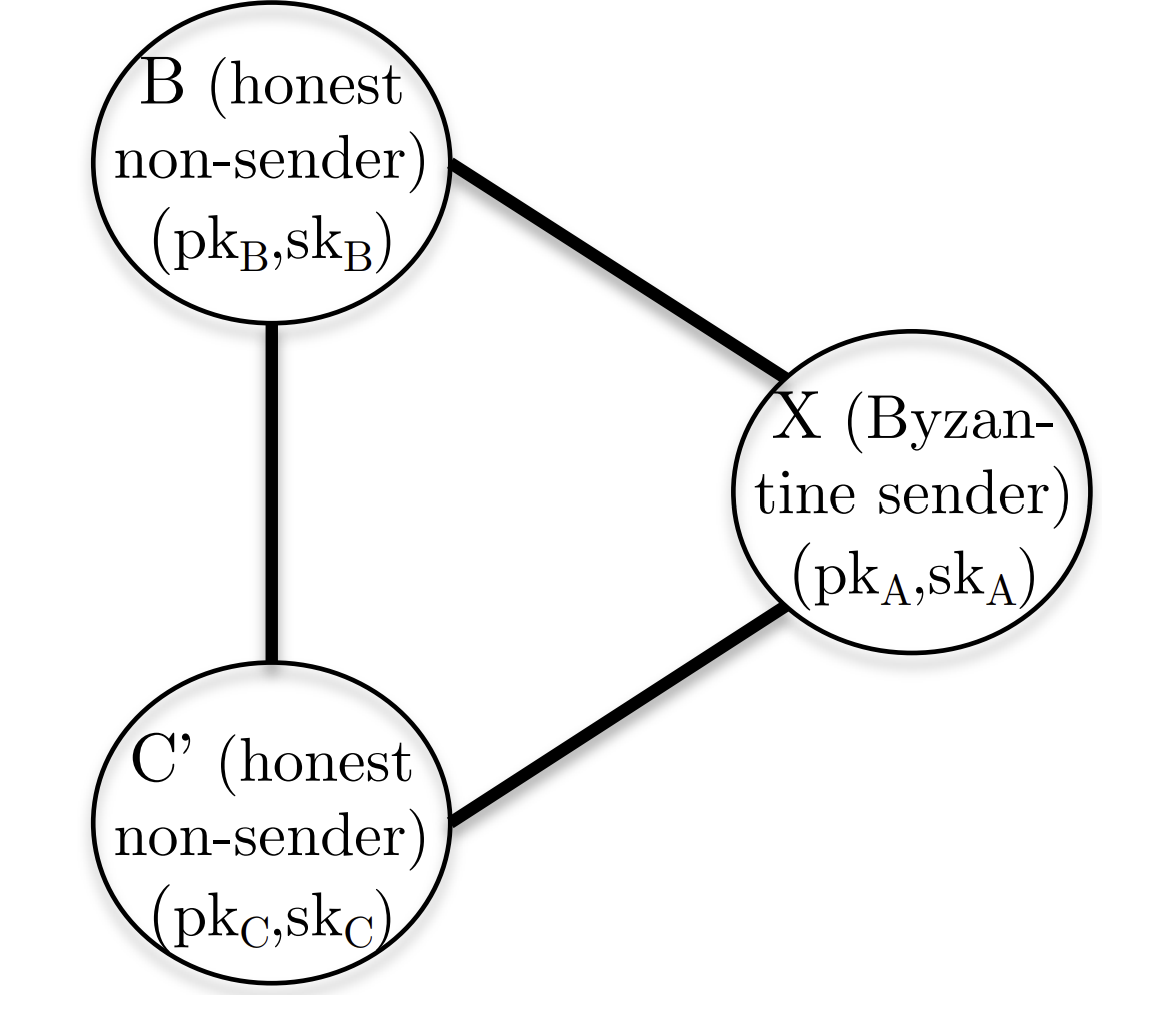
\includegraphics[width=7cm]{figures/f12.png} }}%
    \qquad
    \subfloat[\centering Hexagon thought experiment]{{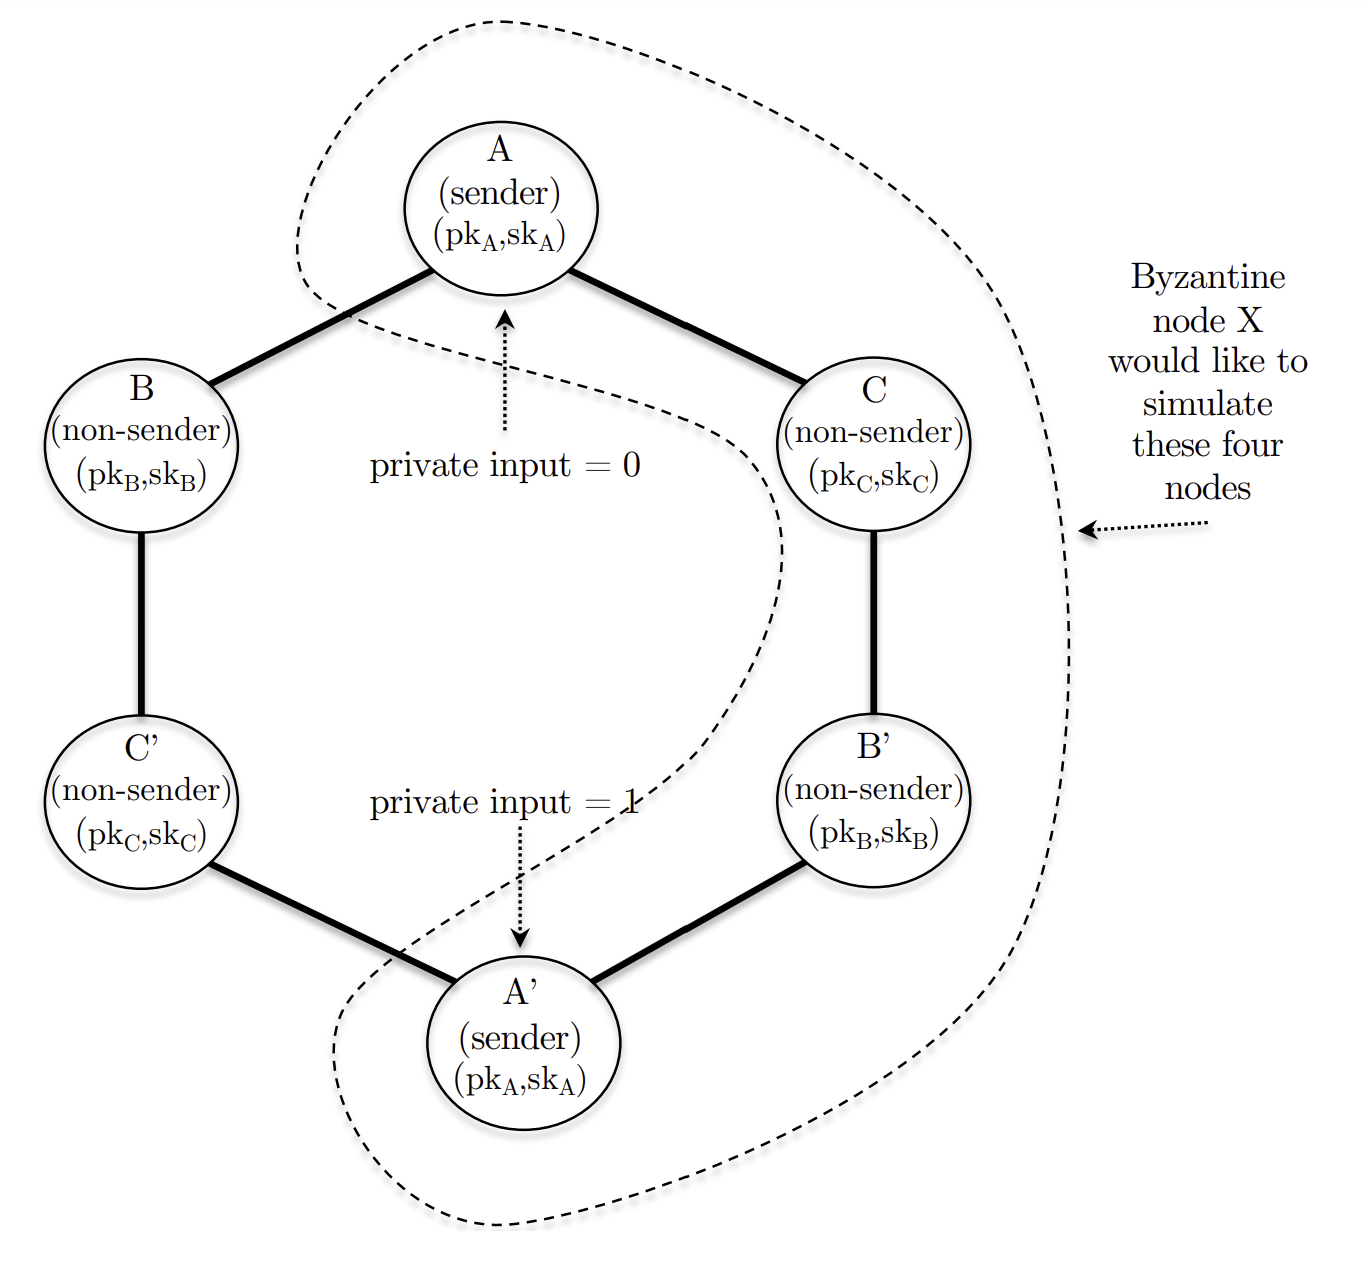
\includegraphics[width=7cm]{figures/f13.png} }}%
    \caption{ An attempt to extend the argument of Figure 3.3 to the PKI setting. The simulation
    strategy could require the forging of signatures without knowledge of the appropriate private
    key, and so the Byzantine node $X$ cannot carry it out.
        }
    \label{fig:example}%
\end{figure}


\subsection{Cryptography and Trusted Setups Matter!}
The fact that there are things you can do with the PKI assumption (the main result of
last lecture) and also things that you pronably cannot do without it (the main result of this lecture) is
super-interesting. We now understand that assumptions about the existence of secure digital
signature schemes and public key distribution fundamentally affects what you can and cannot
do with a consensus protocol.\\
For a point of contrast, think about algorithms. If you’re trying to design a faster
algorithm for the minimum spanning tree problem, who cares what kind of cryptography
exists? Or suppose you are in the middle of tackling an \textit{NP}-hard problem like the traveling
salesman problem, and I hand you on a silver platter a secure digital signature scheme (or
some more fancy cryptographic primitive). You would stare at me quizzically: “What am I
supposed to do this this?” Whereas, for the design of distributed protocols, cryptographic
assumptions fundamentally change the game and enable solutions that otherwise would not
exist.\\
Way back in Section 3.1 we mentioned that one purpose (among many) of impossibility
results is to indicate when you’re working in a too demanding model, with too few assumptions. This lecture’s main result is a textbook example. It shows that, if you want
a consensus protocol that is robust to an arbitrary number of faulty nodes, you have no
choice but to get your hands on a secure digital signature scheme and figure out how to get
everyone’s public keys to everyone else (or pull off some other trusted setup assumption that
makes simulation strategies infeasible for Byzantine nodes). The impossibility result in the
next two lectures (in which we drop the assumption of the synchronous setting) is another
textbook example. Though rather than educating us about the need for trusted setup assumptions, it will guide us toward necessary assumptions on the reliability of the underlying communication network.

\begingroup
\let\clearpage\relax
\begin{thebibliography}{5}
\bibitem{texbook}
M. J. Fischer, N. A. Lynch, and M. Merritt. Easy impossibility proofs for distributed
consensus problems.\textit{ Distributed Computing}, 1(1):26–39, 1986. URL: https://groups.
csail.mit.edu/tds/papers/Lynch/FischerLynchMerritt-dc.pdf.

\bibitem{lamport94}
R. L. Graham and A. C. Yao. On the improbability of reaching Byzantine agreements. In
\textit{Proceedings of the 21st Annual ACM Symposium on Theory of Computing (STOC)}, pages
467–478, 1989. URL: https://mathweb.ucsd.edu/~ronspubs/89\textunderscore08\textunderscore byzantine.pdf.

\bibitem{Mark Schmidt}MM. Pease, R. Shostak, and L. Lamport. Reaching agreement in the presence of faults.
\textit{Journal of the ACM}, 27(2):228–234, 1980. URL: https://lamport.azurewebsites.
net/pubs/reaching.pdf.

\bibitem{fff}T. Roughgarden. \textit{Algorithms Illuminated, Part 4: Algorithms for NP-Hard Problems}.
Soundlikeyourself Publishing, 2020.

\bibitem{fff2}A. Turing. On computable numbers, with an application to the Entscheidungsproblem.
\textit{Proceedings of the London Mathematical Society, Series 2}, 42:230–265, 1936. Erratum:
43:544–546, 1937. URL: https://www.astro.puc.cl/~rparra/tools/PAPERS/turing\textunderscore1936.pdf.
\end{thebibliography}
\endgroup








